\documentclass[11pt,letterpaper,twocolumn]{article}

% ── Packages ──────────────────────────────────────────────
\usepackage[margin=0.85in]{geometry}
\usepackage[T1]{fontenc}
\usepackage{lmodern}
\usepackage{microtype}
\usepackage{graphicx}
\usepackage{xcolor}
\usepackage{tikz}
\usetikzlibrary{arrows.meta,positioning,shapes.geometric,fit,calc,
                 decorations.pathreplacing,backgrounds,patterns}
\usepackage{pgfplots}
\pgfplotsset{compat=1.18}
\usepackage{booktabs}
\usepackage{tabularx}
\usepackage{enumitem}
\usepackage{amsmath}
\usepackage{hyperref}
\usepackage{caption}
\usepackage{subcaption}
\usepackage{float}
\usepackage{multicol}
\usepackage{fancyhdr}
\usepackage{titlesec}

% ── Brand Colors ──────────────────────────────────────────
\definecolor{garnet}{HTML}{73000A}
\definecolor{rose}{HTML}{CC2E40}
\definecolor{atlantic}{HTML}{466A9F}
\definecolor{congaree}{HTML}{1F414D}
\definecolor{horseshoe}{HTML}{65780B}
\definecolor{grass}{HTML}{CED318}
\definecolor{honeycomb}{HTML}{A49137}
\definecolor{warmgrey}{HTML}{676156}
\definecolor{sandstorm}{HTML}{FFF2E3}
\definecolor{bk90}{HTML}{363636}
\definecolor{bk70}{HTML}{5C5C5C}
\definecolor{bk50}{HTML}{A2A2A2}
\definecolor{bk30}{HTML}{C7C7C7}
\definecolor{bk10}{HTML}{ECECEC}

% ── Hyperref config ───────────────────────────────────────
\hypersetup{
  colorlinks=true,
  linkcolor=garnet,
  citecolor=atlantic,
  urlcolor=congaree,
}

% ── Section styling ───────────────────────────────────────
\titleformat{\section}{\large\bfseries\color{garnet}}{\thesection}{0.8em}{}
\titleformat{\subsection}{\normalsize\bfseries\color{congaree}}{\thesubsection}{0.6em}{}
\titleformat{\subsubsection}{\normalsize\itshape\color{bk70}}{\thesubsubsection}{0.6em}{}

% ── Header / Footer ──────────────────────────────────────
\pagestyle{fancy}
\fancyhf{}
\fancyhead[L]{\small\color{bk70}Sub-Agent Architectures}
\fancyhead[R]{\small\color{bk70}J.C.\ Vaught}
\fancyfoot[C]{\small\color{bk50}\thepage}
\renewcommand{\headrulewidth}{0.4pt}
\renewcommand{\headrule}{\hbox to\headwidth{\color{garnet}\leaders\hrule height \headrulewidth\hfill}}

% ── TikZ styles ───────────────────────────────────────────
\tikzset{
  agentbox/.style={
    rectangle, draw=#1, fill=#1!8, thick,
    minimum width=2.2cm, minimum height=0.8cm,
    font=\small\sffamily, align=center,
    inner sep=4pt
  },
  agentbox/.default=garnet,
  workerbox/.style={
    rectangle, draw=atlantic, fill=atlantic!8, thick,
    minimum width=1.8cm, minimum height=0.7cm,
    font=\small\sffamily, align=center,
    inner sep=3pt
  },
  tierbox/.style={
    rectangle, draw=#1, fill=#1!5, thick,
    minimum width=6.5cm, minimum height=1.0cm,
    font=\small\sffamily, align=center,
    inner sep=4pt
  },
  tierbox/.default=garnet,
  dataarrow/.style={
    -{Stealth[length=5pt]}, thick, color=#1
  },
  dataarrow/.default=bk70,
  brace/.style={
    decorate, decoration={brace, amplitude=6pt, raise=2pt}, thick, color=#1
  },
  brace/.default=bk50,
  labelnode/.style={
    font=\scriptsize\sffamily, color=bk70
  },
}

% ══════════════════════════════════════════════════════════
\title{\textcolor{garnet}{\textbf{Sub-Agent Architectures for\\
  Autonomous AI Systems}}\\[6pt]
  \large\textcolor{bk70}{Principles, Patterns, and Research Applications}}
\author{J.C.\ Vaught\\
  \small University of South Carolina\\
  \small\texttt{jvaught@sc.edu}}
\date{\today}

\begin{document}
\maketitle
\thispagestyle{fancy}

% ──────────────────────────────────────────────────────────
\begin{abstract}
\noindent
Large language model (LLM) agents are increasingly deployed as autonomous
systems capable of planning, tool use, and code generation.  A single
monolithic agent, however, faces hard limits: finite context windows, loss of
focus on long tasks, and an inability to specialize.  \textbf{Sub-agent
architectures} address these constraints by decomposing work across multiple
coordinated agents, each with its own context budget and domain focus.  This
document provides a comprehensive treatment of sub-agent design---from
two-layer orchestration to hierarchical multi-tier systems---and examines how
these patterns apply to academic research workflows including literature
review, experimental design, data analysis, and manuscript preparation.
\end{abstract}

% ══════════════════════════════════════════════════════════
\section{Introduction}
\label{sec:intro}

Modern LLM-based coding agents such as Claude Code, OpenHands, and Aider
operate within a single context window, typically 200K tokens.  While
impressive, this budget is consumed rapidly when an agent must simultaneously
reason about strategy, manage state, read large codebases, and produce
output.  The result is a \emph{context bottleneck}: as task complexity grows
linearly, effective context availability shrinks super-linearly due to
attention dilution and retrieval degradation.

Sub-agent architectures resolve this by splitting cognition across multiple
independent agents, each receiving a fresh context window.  The benefits are
threefold:

\begin{enumerate}[leftmargin=*,itemsep=2pt]
  \item \textbf{Specialization.}  Each agent focuses on a narrow domain,
    improving depth of reasoning.
  \item \textbf{Parallelism.}  Independent tasks execute simultaneously,
    yielding 2--8$\times$ wall-clock speedups.
  \item \textbf{Scalability.}  Total available context scales linearly with
    the number of agents spawned.
\end{enumerate}

This document proceeds as follows: Section~\ref{sec:fundamentals} defines
core terminology.  Section~\ref{sec:twolayer} presents the foundational
two-layer pattern.  Section~\ref{sec:multitier} extends to three-tier and
hierarchical designs.  Section~\ref{sec:parallel} covers parallelization
strategies.  Section~\ref{sec:orchestration} details orchestration patterns.
Section~\ref{sec:research} maps these architectures onto research workflows.
Section~\ref{sec:practical} provides implementation guidance, and
Section~\ref{sec:limits} discusses limitations.

% ══════════════════════════════════════════════════════════
\section{Fundamental Concepts}
\label{sec:fundamentals}

\subsection{What Is a Sub-Agent?}

A \textbf{sub-agent} is an LLM invocation spawned by a parent agent to
perform a scoped piece of work.  The sub-agent receives its own system
prompt, context, and tool access.  It executes autonomously and returns a
structured result to its parent.  Critically, the sub-agent's context window
is \emph{independent}---it does not consume tokens from the parent's budget.

\subsection{Tasks vs.\ Subagents}

Two distinct primitives exist for delegating work, and the choice between
them shapes system behavior significantly.

\begin{table}[H]
\centering
\caption{Comparison of task and subagent primitives.}
\label{tab:task-vs-subagent}
\small
\begin{tabularx}{\columnwidth}{@{}lXX@{}}
\toprule
\textbf{Property} & \textbf{Task} & \textbf{Subagent} \\
\midrule
Lifetime    & Ephemeral       & Persistent \\
Context     & 200K, isolated  & Fresh per turn \\
State       & Stateless       & Maintains memory \\
Concurrency & Up to 10        & Typically 1--3 \\
Ideal for   & Parallel, independent work & Iterative, multi-turn work \\
\bottomrule
\end{tabularx}
\end{table}

\textbf{Tasks} are fire-and-forget: the parent issues a prompt, the task
agent executes, and a result is returned.  There is no back-and-forth.
\textbf{Subagents} persist across multiple interactions, enabling iterative
refinement---useful when the output of one step informs the next.

\begin{figure}[H]
\centering
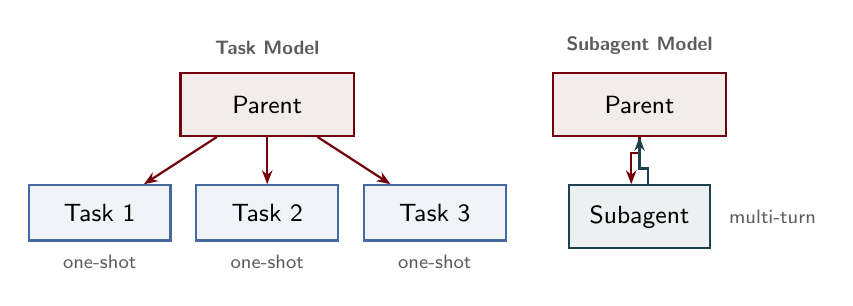
\begin{tikzpicture}[node distance=0.5cm and 0.8cm]
  % Task side
  \node[agentbox=garnet] (parent1) {Parent};
  \node[workerbox, below left=0.6cm and 0.1cm of parent1] (t1) {Task 1};
  \node[workerbox, below=0.6cm of parent1] (t2) {Task 2};
  \node[workerbox, below right=0.6cm and 0.1cm of parent1] (t3) {Task 3};
  \draw[dataarrow=garnet] (parent1) -- (t1);
  \draw[dataarrow=garnet] (parent1) -- (t2);
  \draw[dataarrow=garnet] (parent1) -- (t3);
  \node[labelnode, above=0.1cm of parent1] {\textbf{Task Model}};
  \node[labelnode, below=0.05cm of t1] {one-shot};
  \node[labelnode, below=0.05cm of t2] {one-shot};
  \node[labelnode, below=0.05cm of t3] {one-shot};

  % Subagent side
  \node[agentbox=garnet, right=2.5cm of parent1] (parent2) {Parent};
  \node[agentbox=congaree, below=0.6cm of parent2,
        minimum width=1.8cm] (sub) {Subagent};
  \draw[dataarrow=garnet] (parent2.south) -- ++(0,-0.2) -| ([xshift=-3pt]sub.north);
  \draw[dataarrow=congaree] ([xshift=3pt]sub.north) -- ++(0,0.2) -| (parent2.south);
  \node[labelnode, above=0.1cm of parent2] {\textbf{Subagent Model}};
  \node[labelnode, right=0.1cm of sub] {multi-turn};
\end{tikzpicture}
\caption{Task (left) vs.\ subagent (right) delegation.  Tasks are
  one-shot and parallelizable; subagents support iterative dialogue.}
\label{fig:task-vs-subagent}
\end{figure}

\subsection{The Context Window Constraint}

Every LLM call operates within a fixed context window $C$ (e.g., 200K
tokens).  A single-agent approach must fit planning, code, tool output, and
reasoning into one window:
\[
  C_{\text{effective}} = C - C_{\text{system}} - C_{\text{history}}
  - C_{\text{tools}}
\]
As conversations grow, $C_{\text{history}}$ dominates, leaving little room
for new reasoning.  Sub-agents reset this equation: each receives the full
$C$ budget, minus only the context explicitly passed to it.

% ══════════════════════════════════════════════════════════
\section{Two-Layer Architecture}
\label{sec:twolayer}

The simplest and most widely used sub-agent pattern consists of two layers:
an \textbf{orchestrator} (the main agent) and one or more \textbf{workers}
(task agents).

\subsection{Orchestrator Responsibilities}

The orchestrator follows a five-phase cycle:

\begin{enumerate}[leftmargin=*,itemsep=1pt]
  \item \textbf{Understand:} Parse the user request and identify scope.
  \item \textbf{Plan:} Decompose into atomic, independently executable
    tasks.
  \item \textbf{Spawn:} Create workers with clear instructions, context
    files, and success criteria.
  \item \textbf{Wait:} Collect results; handle timeouts and failures.
  \item \textbf{Synthesize:} Merge worker outputs into a coherent final
    result.
\end{enumerate}

\begin{figure}[H]
\centering
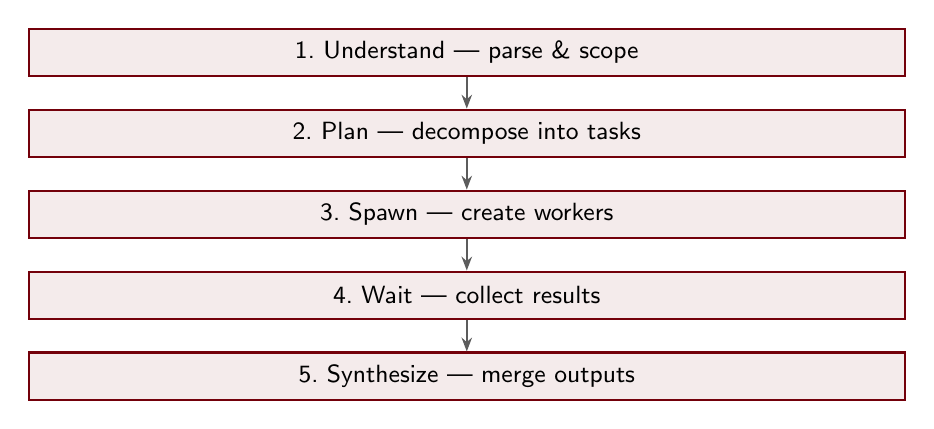
\begin{tikzpicture}[node distance=0.4cm,
  phase/.style={rectangle, draw=garnet, fill=garnet!8, thick,
    minimum width=\columnwidth-1cm, minimum height=0.6cm,
    font=\small\sffamily, align=center}]
  \node[phase] (u) {1.\ Understand --- parse \& scope};
  \node[phase, below=of u] (p) {2.\ Plan --- decompose into tasks};
  \node[phase, below=of p] (s) {3.\ Spawn --- create workers};
  \node[phase, below=of s] (w) {4.\ Wait --- collect results};
  \node[phase, below=of w] (sy) {5.\ Synthesize --- merge outputs};
  \draw[dataarrow] (u) -- (p);
  \draw[dataarrow] (p) -- (s);
  \draw[dataarrow] (s) -- (w);
  \draw[dataarrow] (w) -- (sy);
\end{tikzpicture}
\caption{The five-phase orchestrator cycle.}
\label{fig:orchestrator-cycle}
\end{figure}

\subsection{Worker Lifecycle}

Each worker follows a simpler four-step protocol:

\begin{enumerate}[leftmargin=*,itemsep=1pt]
  \item \textbf{Understand:} Read the task instructions and provided
    context.
  \item \textbf{Execute:} Perform the scoped work using available tools.
  \item \textbf{Validate:} Check output against the success criteria.
  \item \textbf{Report:} Return structured findings to the orchestrator.
\end{enumerate}

The worker must stay within its assigned scope.  It does not modify files
outside its mandate, does not communicate with other workers, and does not
escalate decisions---it either succeeds or reports failure.

\subsection{Communication Flow}

Information flows in two directions with strict filtering:

\begin{itemize}[leftmargin=*,itemsep=1pt]
  \item \textbf{Downward} (orchestrator $\to$ worker): task definition,
    relevant context, constraints, output format specification.
  \item \textbf{Upward} (worker $\to$ orchestrator): outcome status,
    findings, confidence level, recommendations.
\end{itemize}

The orchestrator never sends its full state downward, and workers never send
their full reasoning trace upward.  This \emph{information filtering} is
essential to preserve context budgets.

\begin{figure}[H]
\centering
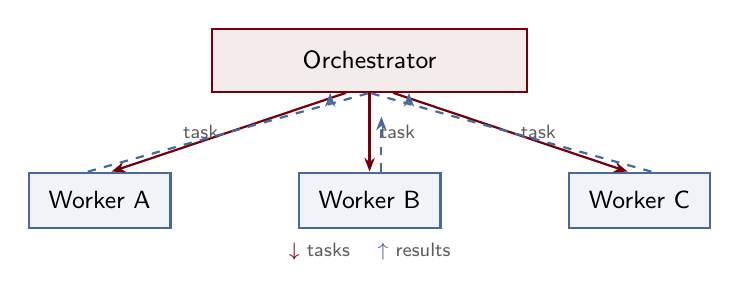
\begin{tikzpicture}[node distance=0.6cm and 0.3cm]
  \node[agentbox=garnet, minimum width=4cm] (orch) {Orchestrator};

  \node[workerbox, below left=1.0cm and 0.5cm of orch] (w1) {Worker A};
  \node[workerbox, below=1.0cm of orch] (w2) {Worker B};
  \node[workerbox, below right=1.0cm and 0.5cm of orch] (w3) {Worker C};

  % Downward arrows
  \draw[dataarrow=garnet] (orch.south) +(-0.3,0) -- ([xshift=0.15cm]w1.north)
    node[midway, left, labelnode] {task};
  \draw[dataarrow=garnet] (orch.south) -- (w2.north)
    node[midway, right, labelnode] {task};
  \draw[dataarrow=garnet] (orch.south) +(0.3,0) -- ([xshift=-0.15cm]w3.north)
    node[midway, right, labelnode] {task};

  % Upward arrows (dashed)
  \draw[dataarrow=atlantic, dashed] ([xshift=-0.15cm]w1.north) -- (orch.south)
    +(-0.5,0);
  \draw[dataarrow=atlantic, dashed] (w2.north) ++(0.15,0) -- ++(0,0.7);
  \draw[dataarrow=atlantic, dashed] ([xshift=0.15cm]w3.north) -- (orch.south)
    +(0.5,0);

  \node[labelnode, below=0.05cm of w2]
    {\textcolor{garnet}{$\downarrow$} tasks \quad
     \textcolor{atlantic}{$\uparrow$} results};
\end{tikzpicture}
\caption{Two-layer communication: the orchestrator delegates tasks
  downward (solid) and receives results upward (dashed).}
\label{fig:twolayer-comm}
\end{figure}

\subsection{Dependency Patterns}

Not all tasks are independent.  Three canonical dependency patterns govern
how workers are scheduled:

\begin{description}[leftmargin=0pt,itemsep=3pt]
  \item[Parallel.] No dependencies---all tasks run simultaneously.  This
    maximizes speedup.
  \item[Linear.] Task $B$ depends on $A$'s output, $C$ depends on $B$, etc.
    Execution is sequential.
  \item[Tree.] Mixed: some tasks run in parallel, their outputs feed into
    dependent tasks.  This is the most common real-world pattern.
\end{description}

\begin{figure}[H]
\centering
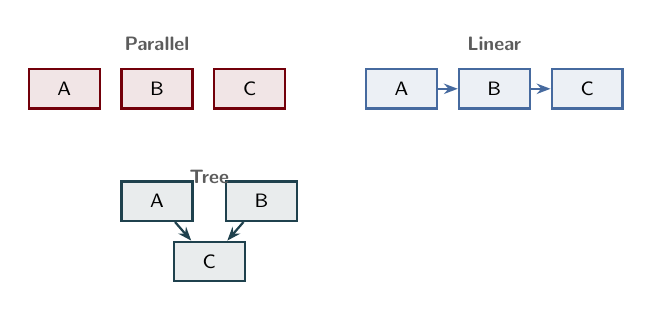
\begin{tikzpicture}[node distance=0.4cm and 0.25cm,
  tsk/.style={rectangle, draw=#1, fill=#1!10, thick,
    minimum width=0.9cm, minimum height=0.5cm,
    font=\scriptsize\sffamily}]

  % Parallel
  \node[tsk=garnet] (p1) {A};
  \node[tsk=garnet, right=of p1] (p2) {B};
  \node[tsk=garnet, right=of p2] (p3) {C};
  \node[labelnode, above=0.1cm of p2] {\textbf{Parallel}};

  % Linear
  \node[tsk=atlantic, right=1.0cm of p3] (l1) {A};
  \node[tsk=atlantic, right=of l1] (l2) {B};
  \node[tsk=atlantic, right=of l2] (l3) {C};
  \draw[dataarrow=atlantic] (l1) -- (l2);
  \draw[dataarrow=atlantic] (l2) -- (l3);
  \node[labelnode, above=0.1cm of l2] {\textbf{Linear}};

  % Tree
  \node[tsk=congaree, below=0.9cm of p2] (t1) {A};
  \node[tsk=congaree, right=0.4cm of t1] (t2) {B};
  \node[tsk=congaree, below=0.5cm of $(t1)!0.5!(t2)$] (t3) {C};
  \draw[dataarrow=congaree] (t1) -- (t3);
  \draw[dataarrow=congaree] (t2) -- (t3);
  \node[labelnode, above=0.1cm of $(t1)!0.5!(t2)$] {\textbf{Tree}};
\end{tikzpicture}
\caption{Three canonical dependency patterns for task scheduling.}
\label{fig:dep-patterns}
\end{figure}

\subsection{Error Handling}

Workers can fail for several reasons: timeout, out-of-memory, malformed
output, or logical errors.  The orchestrator applies graduated recovery:

\begin{enumerate}[leftmargin=*,itemsep=1pt]
  \item \textbf{Retry} the task with a refined prompt or additional context.
  \item \textbf{Decompose} further---the task may have been too broad.
  \item \textbf{Partial results}---use what succeeded and note the gap.
  \item \textbf{Escalate}---if multiple workers fail on the same task,
    flag a systemic issue to the user.
\end{enumerate}

% ══════════════════════════════════════════════════════════
\section{Multi-Tier Architectures}
\label{sec:multitier}

\subsection{The Three-Tier Foundation}

For complex projects, two layers are insufficient.  The three-tier
architecture inserts a \textbf{planning layer} between strategy and
execution:

\begin{figure}[H]
\centering
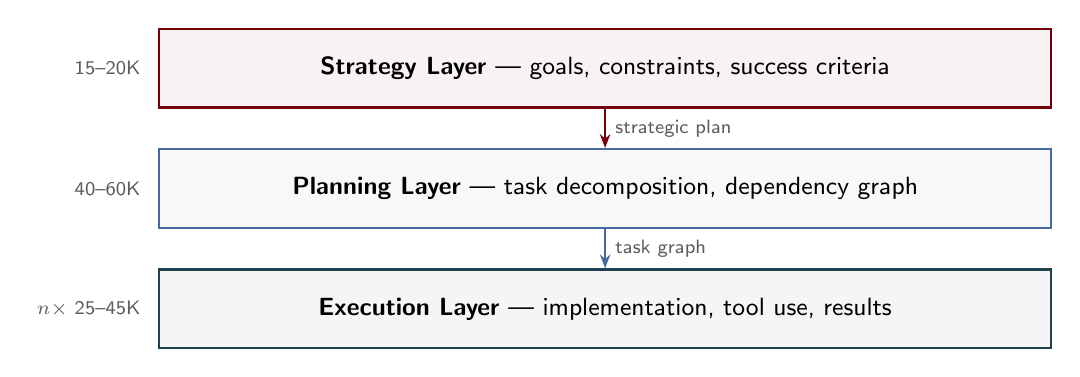
\begin{tikzpicture}[node distance=0.5cm]
  \node[tierbox=garnet, minimum width=\columnwidth-0.8cm] (strat)
    {\textbf{Strategy Layer} --- goals, constraints, success criteria};
  \node[tierbox=atlantic, minimum width=\columnwidth-0.8cm, below=of strat] (plan)
    {\textbf{Planning Layer} --- task decomposition, dependency graph};
  \node[tierbox=congaree, minimum width=\columnwidth-0.8cm, below=of plan] (exec)
    {\textbf{Execution Layer} --- implementation, tool use, results};

  \draw[dataarrow=garnet] (strat) -- (plan)
    node[midway, right, labelnode] {strategic plan};
  \draw[dataarrow=atlantic] (plan) -- (exec)
    node[midway, right, labelnode] {task graph};

  % Token annotations
  \node[labelnode, left=0.1cm of strat] {15--20K};
  \node[labelnode, left=0.1cm of plan] {40--60K};
  \node[labelnode, left=0.1cm of exec] {$n \times$ 25--45K};
\end{tikzpicture}
\caption{Three-tier architecture with typical token budgets per layer.
  The execution layer runs multiple agents in parallel.}
\label{fig:three-tier}
\end{figure}

\textbf{Why three tiers?}  The strategy layer reasons about \emph{what} to
accomplish; the planning layer determines \emph{how} to decompose it; and the
execution layer performs the actual work.  This separation prevents the
strategy agent from being overwhelmed by implementation details, and prevents
execution agents from making strategic decisions they lack context for.

\subsubsection{Token Budget Scaling}

Total token consumption for a three-tier system with $n$ execution agents:
\[
  T_{\text{total}} = T_{\text{strategy}} + T_{\text{planning}}
    + n \cdot T_{\text{execution}}
\]
For $n = 5$ agents, a typical budget is $15\text{K} + 50\text{K} + 5 \times
35\text{K} = 240\text{K}$ tokens---far exceeding what a single 200K-context
agent can achieve.

\subsection{Hierarchical Multi-Agent Systems}

For very large problems, the three-tier model generalizes to an
\textbf{arbitrary-depth hierarchy}.  A root agent (the ``chief architect'')
delegates to domain leads, who in turn delegate to specialists.

\begin{figure}[H]
\centering
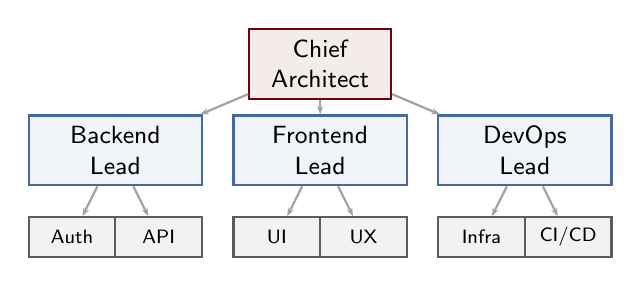
\begin{tikzpicture}[
  level 1/.style={sibling distance=2.6cm, level distance=1.1cm},
  level 2/.style={sibling distance=1.1cm, level distance=1.1cm},
  every node/.style={agentbox=bk70, minimum width=1.1cm,
    minimum height=0.5cm, font=\scriptsize\sffamily, inner sep=2pt},
  edge from parent/.style={draw=bk50, thick, -{Stealth[length=3pt]}}
]
  \node[agentbox=garnet, minimum width=1.8cm] {Chief\\Architect}
    child { node[agentbox=atlantic] {Backend\\Lead}
      child { node {Auth} }
      child { node {API} }
    }
    child { node[agentbox=atlantic] {Frontend\\Lead}
      child { node {UI} }
      child { node {UX} }
    }
    child { node[agentbox=atlantic] {DevOps\\Lead}
      child { node {Infra} }
      child { node {CI/CD} }
    };
\end{tikzpicture}
\caption{Hierarchical multi-agent system.  Domain leads coordinate
  specialists; the root agent coordinates leads.}
\label{fig:hmas}
\end{figure}

\subsubsection{Depth Limitations}

Each level of nesting multiplies total token cost and adds latency.
Empirically, the practical limit is \textbf{3--4 levels}:

\begin{table}[H]
\centering
\caption{Token scaling with hierarchy depth (2 children per node).}
\label{tab:depth-tokens}
\small
\begin{tabular}{@{}ccc@{}}
\toprule
\textbf{Depth} & \textbf{Agents} & \textbf{Total Tokens} \\
\midrule
1 & 1   & 50K \\
2 & 3   & 100K \\
3 & 7   & 200K \\
4 & 15  & 400K \\
5 & 31  & 800K+ (overflow) \\
\bottomrule
\end{tabular}
\end{table}

Beyond depth 4, coordination overhead, context contamination, and latency
make deeper hierarchies impractical.  Instead, use \emph{flat delegation}
(all coordination at one level) or \emph{file-mediated pipelines}
(Agent $\to$ File $\to$ Agent).

\subsection{Leader-Worker Load Balancing}

When many similar tasks must be processed, a \textbf{leader-worker pool}
distributes work across a fixed or dynamic set of workers.

\begin{figure}[H]
\centering
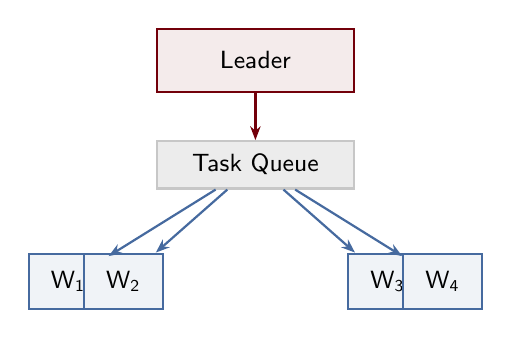
\begin{tikzpicture}[node distance=0.4cm and 0.5cm]
  \node[agentbox=garnet, minimum width=2.5cm] (leader) {Leader};
  \node[rectangle, draw=bk30, fill=bk10, thick,
    minimum width=2.5cm, minimum height=0.6cm,
    below=0.6cm of leader, font=\small\sffamily] (queue) {Task Queue};

  \node[workerbox, below left=0.8cm and 0.6cm of queue, minimum width=1.0cm]
    (w1) {W\textsubscript{1}};
  \node[workerbox, below left=0.8cm and -0.1cm of queue, minimum width=1.0cm]
    (w2) {W\textsubscript{2}};
  \node[workerbox, below right=0.8cm and -0.1cm of queue, minimum width=1.0cm]
    (w3) {W\textsubscript{3}};
  \node[workerbox, below right=0.8cm and 0.6cm of queue, minimum width=1.0cm]
    (w4) {W\textsubscript{4}};

  \draw[dataarrow=garnet] (leader) -- (queue);
  \draw[dataarrow=atlantic] (queue) -- (w1);
  \draw[dataarrow=atlantic] (queue) -- (w2);
  \draw[dataarrow=atlantic] (queue) -- (w3);
  \draw[dataarrow=atlantic] (queue) -- (w4);
\end{tikzpicture}
\caption{Leader-worker pool with a shared task queue.  The leader
  enqueues tasks; workers dequeue and execute.}
\label{fig:leader-worker}
\end{figure}

Common load-balancing strategies include round-robin (simple, fair),
work-stealing queues (adaptive), priority queues (latency-optimized), and
capacity-based assignment (balanced utilization).

% ══════════════════════════════════════════════════════════
\section{Parallelization}
\label{sec:parallel}

\subsection{Performance Impact}

Parallelization delivers substantial improvements across task types:

\begin{figure}[H]
\centering
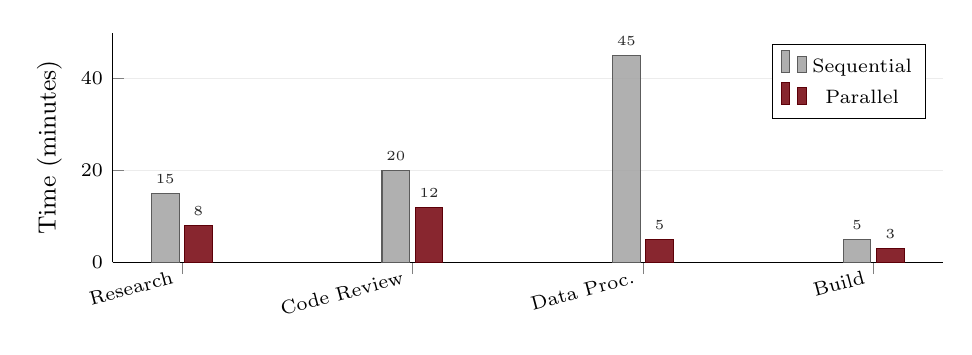
\begin{tikzpicture}
\begin{axis}[
  ybar,
  bar width=10pt,
  width=\columnwidth,
  height=4.5cm,
  ymin=0, ymax=50,
  ylabel={Time (minutes)},
  ylabel style={font=\small},
  symbolic x coords={Research, Code Review, Data Proc., Build},
  xtick=data,
  xticklabel style={font=\scriptsize, rotate=15, anchor=east},
  yticklabel style={font=\scriptsize},
  legend style={font=\scriptsize, at={(0.98,0.95)}, anchor=north east},
  nodes near coords,
  nodes near coords style={font=\tiny},
  every axis plot/.append style={fill opacity=0.85},
  axis lines*=left,
  ymajorgrids=true,
  grid style={bk10, thin},
]
\addplot[fill=bk50, draw=bk70] coordinates
  {(Research,15) (Code Review,20) (Data Proc.,45) (Build,5)};
\addplot[fill=garnet, draw=garnet!80!black] coordinates
  {(Research,8) (Code Review,12) (Data Proc.,5) (Build,3)};
\legend{Sequential, Parallel}
\end{axis}
\end{tikzpicture}
\caption{Wall-clock time comparison: sequential vs.\ parallel execution
  across four task categories.}
\label{fig:perf-comparison}
\end{figure}

The largest gains appear in data processing (60--70\% faster), where tasks
are naturally independent.  Even tightly coupled tasks like code review see
35--45\% improvement through domain-specialized parallel agents.

\subsection{Cost--Speed Tradeoff}

Parallelization is not free: each additional agent consumes its own token
budget.  The tradeoff is:
\[
  \text{Speedup} = \frac{T_{\text{sequential}}}
    {\max(T_{\text{agent}_1}, \ldots, T_{\text{agent}_n})}
  \qquad
  \text{Cost} = n \cdot T_{\text{tokens per agent}}
\]
Parallelism is worthwhile when the time value of the speedup exceeds the
marginal token cost.

\subsection{Synchronization Barriers}

When parallel agents must reconverge, three barrier types apply:

\begin{description}[leftmargin=0pt,itemsep=2pt]
  \item[Full barrier.] Wait for \emph{all} agents.  Used when every result
    is needed.
  \item[Partial barrier ($k$-of-$n$).] Proceed when $k$ of $n$ agents
    finish.  Used for redundant tasks (consensus).
  \item[Timeout barrier.] Wait up to $t$ seconds, then proceed with
    available results.  Used for best-effort tasks.
\end{description}

\subsection{Decision Framework}

\begin{table}[H]
\centering
\caption{When to use parallel vs.\ sequential execution.}
\label{tab:parallel-decision}
\small
\begin{tabularx}{\columnwidth}{@{}lXX@{}}
\toprule
\textbf{Factor} & \textbf{Parallel} & \textbf{Sequential} \\
\midrule
Dependencies   & None between tasks    & Output feeds next task \\
Time           & $> 10$ min sequential & $< 5$ min total \\
Quality        & Multiple perspectives & Single expert suffices \\
Budget         & Token-rich            & Token-constrained \\
Coupling       & Loosely coupled       & Tightly coupled \\
\bottomrule
\end{tabularx}
\end{table}

% ══════════════════════════════════════════════════════════
\section{Orchestration Patterns}
\label{sec:orchestration}

Four canonical orchestration patterns recur across multi-agent systems.  Each
is suited to different problem structures.

\begin{figure*}[t]
\centering
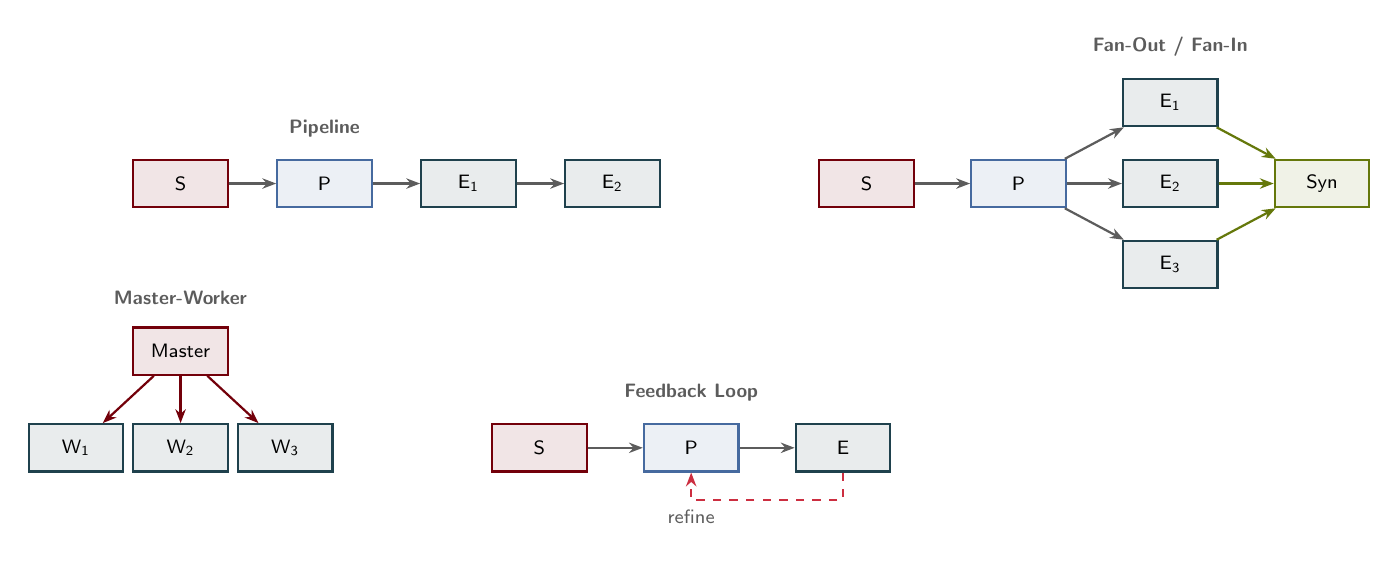
\begin{tikzpicture}[node distance=0.4cm and 0.6cm,
  box/.style={rectangle, draw=#1, fill=#1!10, thick,
    minimum width=1.2cm, minimum height=0.6cm,
    font=\scriptsize\sffamily, align=center},
  box/.default=atlantic]

  % ── Pipeline ────────────────
  \node[box=garnet] (pa) {S};
  \node[box, right=of pa] (pb) {P};
  \node[box=congaree, right=of pb] (pc) {E\textsubscript{1}};
  \node[box=congaree, right=of pc] (pd) {E\textsubscript{2}};
  \draw[dataarrow] (pa) -- (pb);
  \draw[dataarrow] (pb) -- (pc);
  \draw[dataarrow] (pc) -- (pd);
  \node[labelnode, above=0.15cm of pb] {\textbf{Pipeline}};

  % ── Fan-Out / Fan-In ───────
  \node[box=garnet, right=2.0cm of pd] (fo) {S};
  \node[box, right=0.7cm of fo] (fp) {P};
  \node[box=congaree, above right=0.4cm and 0.7cm of fp] (fe1) {E\textsubscript{1}};
  \node[box=congaree, right=0.7cm of fp] (fe2) {E\textsubscript{2}};
  \node[box=congaree, below right=0.4cm and 0.7cm of fp] (fe3) {E\textsubscript{3}};
  \node[box=horseshoe, right=0.7cm of fe2] (syn) {Syn};
  \draw[dataarrow] (fo) -- (fp);
  \draw[dataarrow] (fp) -- (fe1);
  \draw[dataarrow] (fp) -- (fe2);
  \draw[dataarrow] (fp) -- (fe3);
  \draw[dataarrow=horseshoe] (fe1) -- (syn);
  \draw[dataarrow=horseshoe] (fe2) -- (syn);
  \draw[dataarrow=horseshoe] (fe3) -- (syn);
  \node[labelnode, above=0.15cm of fe1]
    {\textbf{Fan-Out / Fan-In}};

  % ── Master-Worker ──────────
  \node[box=garnet, below=1.5cm of pa] (mw) {Master};
  \node[box=congaree, below left=0.6cm and 0.1cm of mw] (mw1)
    {W\textsubscript{1}};
  \node[box=congaree, below=0.6cm of mw] (mw2) {W\textsubscript{2}};
  \node[box=congaree, below right=0.6cm and 0.1cm of mw] (mw3)
    {W\textsubscript{3}};
  \draw[dataarrow=garnet] (mw) -- (mw1);
  \draw[dataarrow=garnet] (mw) -- (mw2);
  \draw[dataarrow=garnet] (mw) -- (mw3);
  \node[labelnode, above=0.15cm of mw] {\textbf{Master-Worker}};

  % ── Feedback Loop ──────────
  \node[box=garnet, right=2.0cm of mw3] (fb) {S};
  \node[box, right=0.7cm of fb] (fbp) {P};
  \node[box=congaree, right=0.7cm of fbp] (fbe) {E};
  \draw[dataarrow] (fb) -- (fbp);
  \draw[dataarrow] (fbp) -- (fbe);
  \draw[dataarrow=rose, thick, dashed]
    (fbe.south) -- ++(0,-0.35) -| (fbp.south)
    node[midway, below, labelnode] {refine};
  \node[labelnode, above=0.15cm of fbp] {\textbf{Feedback Loop}};
\end{tikzpicture}
\caption{Four canonical orchestration patterns.  S = Strategy, P =
  Planning, E = Execution, Syn = Synthesis.  The feedback loop (bottom
  right) enables iterative refinement.}
\label{fig:orch-patterns}
\end{figure*}

\begin{description}[leftmargin=0pt,itemsep=4pt]
  \item[Pipeline.] Strict sequential handoff: Strategy $\to$ Planning $\to$
    Execution$_1$ $\to$ Execution$_2$.  Used when each stage transforms the
    output for the next.

  \item[Fan-Out/Fan-In.] A planner distributes independent tasks to
    parallel workers, then a synthesizer merges results.  This is the most
    common pattern for research tasks.

  \item[Master-Worker.] A master repeatedly distributes similar tasks from
    a queue to a pool of identical workers.  Ideal for batch processing (e.g.,
    analyzing 50 files).

  \item[Feedback Loop.] Execution results flow back to the planner for
    iterative refinement.  Used in debugging, optimization, and any task
    where the first attempt is unlikely to be final.
\end{description}

\subsection{Result Synthesis}

When multiple workers return results, the orchestrator must merge them.  The
synthesis process follows five steps:

\begin{enumerate}[leftmargin=*,itemsep=1pt]
  \item \textbf{Aggregate} all findings into a unified structure.
  \item \textbf{Deduplicate} overlapping results.
  \item \textbf{Prioritize} by severity, confidence, or relevance.
  \item \textbf{Validate} consistency across workers (flag contradictions).
  \item \textbf{Format} the merged result for the end user.
\end{enumerate}

\subsection{Conflict Resolution}

When workers disagree, four resolution strategies are available:

\begin{itemize}[leftmargin=*,itemsep=1pt]
  \item \textbf{Priority-based:} Higher-authority agent wins.
  \item \textbf{Vote-based:} Majority ($k$-of-$n$) consensus.
  \item \textbf{Consequence-based:} Evaluate downstream impact of each
    option.
  \item \textbf{Escalation:} Return the conflict to the user for a
    decision.
\end{itemize}

% ══════════════════════════════════════════════════════════
\section{Research Applications}
\label{sec:research}

Sub-agent architectures map naturally onto the phases of academic research.
This section demonstrates how each architectural pattern accelerates
specific research activities.

\subsection{Literature Review}

A fan-out/fan-in pattern with three specialized agents:

\begin{figure}[H]
\centering
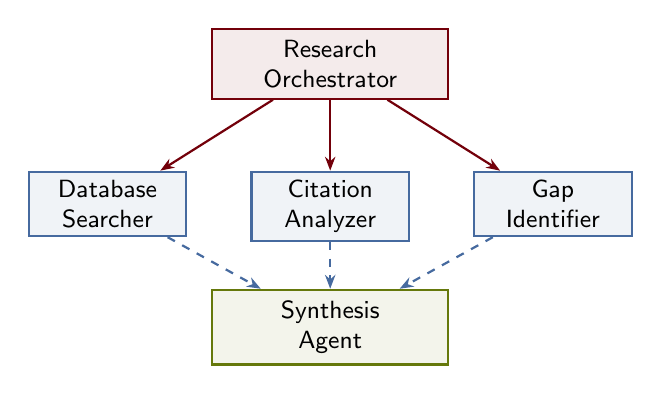
\begin{tikzpicture}[node distance=0.5cm and 0.3cm]
  \node[agentbox=garnet, minimum width=3.0cm] (orch)
    {Research\\Orchestrator};
  \node[workerbox, below left=0.9cm and 0.3cm of orch,
    minimum width=2.0cm] (a1) {Database\\Searcher};
  \node[workerbox, below=0.9cm of orch,
    minimum width=2.0cm] (a2) {Citation\\Analyzer};
  \node[workerbox, below right=0.9cm and 0.3cm of orch,
    minimum width=2.0cm] (a3) {Gap\\Identifier};

  \draw[dataarrow=garnet] (orch) -- (a1);
  \draw[dataarrow=garnet] (orch) -- (a2);
  \draw[dataarrow=garnet] (orch) -- (a3);

  \node[agentbox=horseshoe, below=2.4cm of orch,
    minimum width=3.0cm] (syn) {Synthesis\\Agent};
  \draw[dataarrow=atlantic, dashed] (a1) -- (syn);
  \draw[dataarrow=atlantic, dashed] (a2) -- (syn);
  \draw[dataarrow=atlantic, dashed] (a3) -- (syn);
\end{tikzpicture}
\caption{Literature review with three parallel agents feeding a
  synthesis agent.}
\label{fig:lit-review}
\end{figure}

\begin{itemize}[leftmargin=*,itemsep=1pt]
  \item \textbf{Database Searcher:} Queries academic databases, retrieves
    abstracts, filters by relevance.
  \item \textbf{Citation Analyzer:} Maps citation networks, identifies
    seminal papers and emerging trends.
  \item \textbf{Gap Identifier:} Cross-references findings to identify
    unexplored areas and contradictions.
  \item \textbf{Synthesis Agent:} Merges all findings into a structured
    literature review with taxonomy.
\end{itemize}

\subsection{Experimental Design and Execution}

A three-tier architecture supports the full experimental lifecycle:

\begin{enumerate}[leftmargin=*,itemsep=2pt]
  \item \textbf{Strategy agent} defines hypotheses, variables, and success
    metrics.
  \item \textbf{Planning agent} designs the experimental matrix:
    parameter combinations, data splits, baseline configurations.
  \item \textbf{Execution agents} (parallel) each run one experimental
    configuration, collect metrics, and report results.
\end{enumerate}

For a typical hyperparameter sweep with 20 configurations, 10 parallel
execution agents reduce wall-clock time by $\approx$50\% (2 batches of 10
vs.\ 20 sequential runs).

\subsection{Data Analysis Pipeline}

The master-worker pattern excels at processing large datasets:

\begin{figure}[H]
\centering
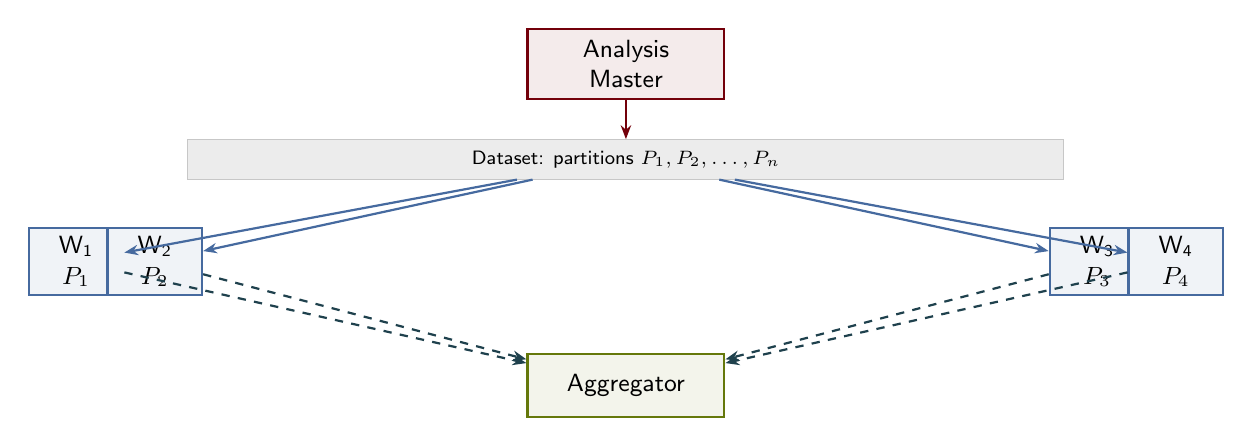
\begin{tikzpicture}[node distance=0.3cm and 0.2cm]
  \node[agentbox=garnet, minimum width=2.5cm] (master) {Analysis\\Master};

  % Data partitions
  \node[rectangle, draw=bk30, fill=bk10,
    minimum width=\columnwidth-1cm, minimum height=0.5cm,
    below=0.5cm of master, font=\scriptsize\sffamily] (data)
    {Dataset: partitions $P_1, P_2, \ldots, P_n$};

  \node[workerbox, below left=0.6cm and 0.8cm of data, minimum width=1.2cm]
    (w1) {W\textsubscript{1}\\$P_1$};
  \node[workerbox, below left=0.6cm and -0.2cm of data, minimum width=1.2cm]
    (w2) {W\textsubscript{2}\\$P_2$};
  \node[workerbox, below right=0.6cm and -0.2cm of data, minimum width=1.2cm]
    (w3) {W\textsubscript{3}\\$P_3$};
  \node[workerbox, below right=0.6cm and 0.8cm of data, minimum width=1.2cm]
    (w4) {W\textsubscript{4}\\$P_4$};

  \draw[dataarrow=garnet] (master) -- (data);
  \draw[dataarrow=atlantic] (data) -- (w1);
  \draw[dataarrow=atlantic] (data) -- (w2);
  \draw[dataarrow=atlantic] (data) -- (w3);
  \draw[dataarrow=atlantic] (data) -- (w4);

  \node[agentbox=horseshoe, below=2.2cm of data, minimum width=2.5cm]
    (agg) {Aggregator};
  \draw[dataarrow=congaree, dashed] (w1) -- (agg);
  \draw[dataarrow=congaree, dashed] (w2) -- (agg);
  \draw[dataarrow=congaree, dashed] (w3) -- (agg);
  \draw[dataarrow=congaree, dashed] (w4) -- (agg);
\end{tikzpicture}
\caption{Data analysis pipeline: a master partitions the dataset and
  distributes to parallel workers.  An aggregator merges results.}
\label{fig:data-pipeline}
\end{figure}

Each worker analyzes its partition independently---computing statistics,
generating visualizations, or running models.  The aggregator then combines
partial results into a global analysis.

\subsection{Manuscript Preparation}

A pipeline pattern supports the writing workflow:

\begin{enumerate}[leftmargin=*,itemsep=1pt]
  \item \textbf{Outline Agent:} Structures the paper (sections, arguments,
    figure placement).
  \item \textbf{Section Writers} (parallel): Each agent writes one section
    with access to relevant data and references.
  \item \textbf{Figure Agent:} Generates plots, diagrams, and tables from
    experimental data.
  \item \textbf{Integration Agent:} Merges sections, ensures narrative
    consistency, formats citations.
  \item \textbf{Review Agent:} Checks for logical gaps, unsupported claims,
    and style issues.
\end{enumerate}

\subsection{Full Research Workflow}

Combining all patterns yields a four-phase research pipeline:

\begin{figure}[H]
\centering
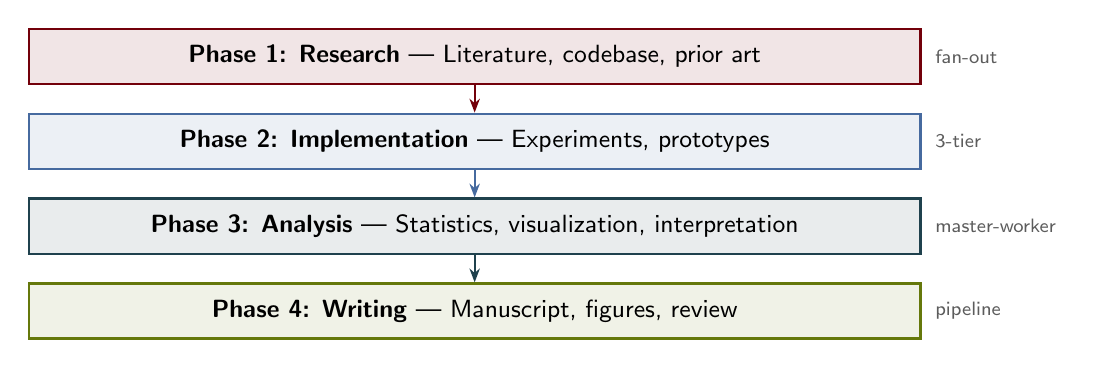
\begin{tikzpicture}[node distance=0.35cm,
  phase/.style={rectangle, draw=#1, fill=#1!10, thick,
    minimum width=\columnwidth-0.8cm, minimum height=0.7cm,
    font=\small\sffamily, align=center},
  phase/.default=garnet]
  \node[phase=garnet] (r) {\textbf{Phase 1: Research} ---
    Literature, codebase, prior art};
  \node[phase=atlantic, below=of r] (i) {\textbf{Phase 2: Implementation}
    --- Experiments, prototypes};
  \node[phase=congaree, below=of i] (a) {\textbf{Phase 3: Analysis} ---
    Statistics, visualization, interpretation};
  \node[phase=horseshoe, below=of a] (w) {\textbf{Phase 4: Writing} ---
    Manuscript, figures, review};

  \draw[dataarrow=garnet] (r) -- (i);
  \draw[dataarrow=atlantic] (i) -- (a);
  \draw[dataarrow=congaree] (a) -- (w);

  % Annotations
  \node[labelnode, right=0.05cm of r] {fan-out};
  \node[labelnode, right=0.05cm of i] {3-tier};
  \node[labelnode, right=0.05cm of a] {master-worker};
  \node[labelnode, right=0.05cm of w] {pipeline};
\end{tikzpicture}
\caption{Full research workflow mapped to orchestration patterns.  Each
  phase uses the pattern best suited to its structure.}
\label{fig:research-workflow}
\end{figure}

% ══════════════════════════════════════════════════════════
\section{Practical Implementation}
\label{sec:practical}

\subsection{Agent Specialization}

Effective sub-agent systems define specialized roles.  Table~\ref{tab:roles}
lists common agent roles for research contexts.

\begin{table}[H]
\centering
\caption{Recommended agent roles for research workflows.}
\label{tab:roles}
\small
\begin{tabularx}{\columnwidth}{@{}lX@{}}
\toprule
\textbf{Role} & \textbf{Responsibility} \\
\midrule
Explorer     & Codebase search, file discovery \\
Researcher   & Literature search, reference gathering \\
Coder        & Implementation, refactoring \\
Analyst      & Statistical analysis, metrics computation \\
Visualizer   & Plot generation, diagram creation \\
Reviewer     & Quality checks, style enforcement \\
Writer       & Prose generation, section drafting \\
\bottomrule
\end{tabularx}
\end{table}

\subsection{Context Provisioning Best Practices}

\begin{enumerate}[leftmargin=*,itemsep=2pt]
  \item \textbf{Minimal context:} Pass only the files and information each
    worker needs---not the entire project.
  \item \textbf{Explicit instructions:} Include success criteria, output
    format, and scope boundaries.
  \item \textbf{File references over content:} Point workers to file paths
    rather than pasting file contents into prompts.
  \item \textbf{Progressive summarization:} When results flow upward,
    summarize rather than forwarding raw output.
\end{enumerate}

\subsection{Batching Strategy}

Most systems cap concurrent agents (e.g., 10 in Claude Code).  For larger
workloads, batch tasks into groups:

\[
  \text{Batches} = \left\lceil \frac{N_{\text{tasks}}}{N_{\text{max concurrent}}} \right\rceil
\]

For 50 tasks with a concurrency limit of 10: 5 sequential batches, each
running 10 tasks in parallel.  Total time $\approx 5 \times
\max(T_{\text{batch}})$, compared to $50 \times T_{\text{task}}$
sequentially.

\subsection{State Management}

Three approaches to managing shared state across agents:

\begin{description}[leftmargin=0pt,itemsep=2pt]
  \item[Centralized.] The orchestrator holds all state.  Simple but creates
    a bottleneck.
  \item[Distributed.] Each agent maintains its own state, synchronized via
    shared files.  Resilient but harder to coordinate.
  \item[Hybrid.] Critical state (e.g., dependency graph, completion
    tracking) is centralized; execution state is distributed.  This is the
    recommended approach.
\end{description}

% ══════════════════════════════════════════════════════════
\section{Limitations and Open Problems}
\label{sec:limits}

\subsection{Token Cost Multiplication}

The primary cost of sub-agent architectures is token consumption.  A system
with 5 parallel agents uses approximately 5$\times$ the tokens of a
single-agent approach.  For token-billed APIs, this directly impacts cost.

\subsection{Coordination Overhead}

Each layer of abstraction adds latency for delegation, result collection, and
synthesis.  For tasks shorter than $\sim$5 minutes, the overhead can
exceed the parallelization benefit.

\subsection{Context Contamination}

When context is passed between agents imprecisely, irrelevant information
accumulates.  This ``context contamination'' degrades downstream agent
performance.  Strict context filtering mitigates but does not eliminate
this problem.

\subsection{Error Propagation}

In deep hierarchies, a failure at a leaf node may not surface until synthesis,
by which time recovery is expensive.  Robust error handling at every level is
essential but adds complexity.

\subsection{Reproducibility}

LLM outputs are inherently stochastic.  Multi-agent systems amplify this
variance: the same input may produce different task decompositions, different
worker assignments, and different final outputs across runs.  For research
applications, this non-determinism must be carefully managed through logging,
seed control, and consensus mechanisms.

% ══════════════════════════════════════════════════════════
\section{Conclusion}

Sub-agent architectures transform single-agent LLM systems into scalable,
specialized, parallel workforces.  The core insight is simple:
\emph{decompose complex problems into scoped tasks, execute them
independently, and synthesize the results.}  The two-layer pattern handles
most use cases; three-tier architectures add a planning layer for complex
projects; and hierarchical systems scale to enterprise-grade problems.

For research applications, these patterns map directly onto established
workflows: literature review (fan-out/fan-in), experimental execution
(three-tier), data analysis (master-worker), and manuscript preparation
(pipeline).  The result is faster iteration, broader coverage, and higher
quality through cross-validation---at the cost of increased token
consumption.

As LLM context windows grow and inference costs decline, the economic case
for sub-agent architectures will only strengthen.  The patterns described
here provide a foundation for building effective multi-agent research systems
today.

\end{document}
